\subsection{Javascript-Client}

\begin{frame}
\begin{center}
	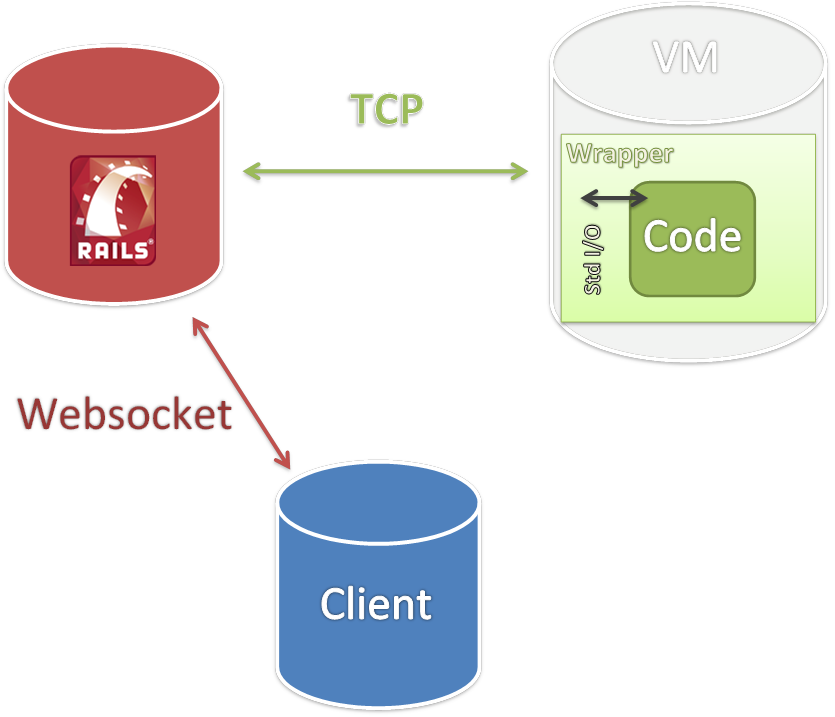
\includegraphics[scale=0.35]{overview}
\end{center}
\end{frame}

\begin{frame}
\frametitle{Web-Technologien}
\begin{center}
	
\includegraphics[scale=0.2]{client/HTML5_Logo.png}
	
\includegraphics[scale=0.2]{client/css3logo.png}
	
\end{center}		
	
	
	
\includegraphics[scale=0.4]{client/coffeescript-logo.png}
	
\includegraphics[scale=0.40]{client/less-logo.png}
	
\includegraphics[scale=0.045]{client/bootstrap-logo.png}
\end{frame}

\begin{frame}
\frametitle{Javascript-Client}
\begin{center}
	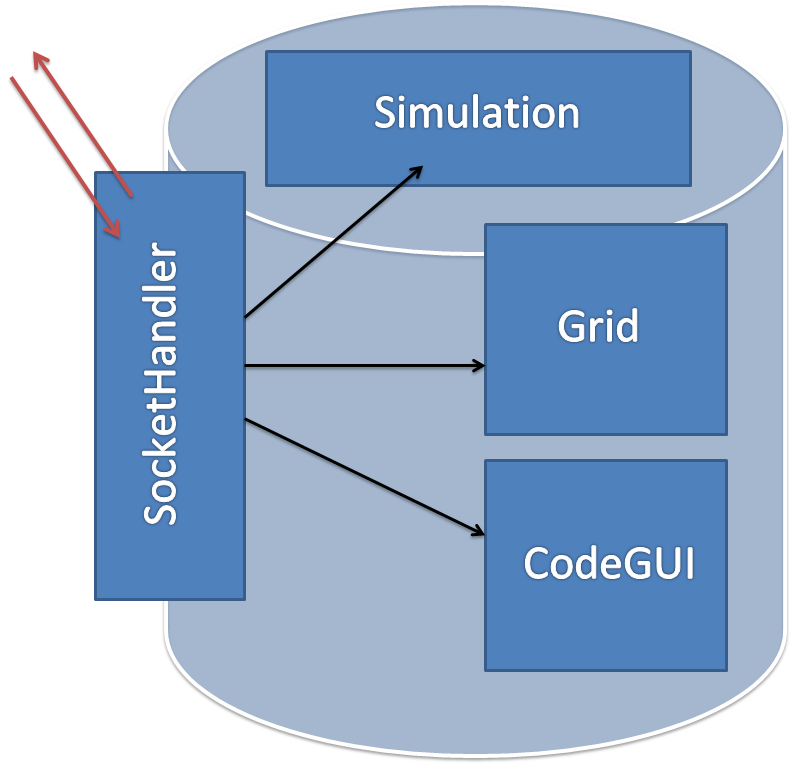
\includegraphics[scale=0.3]{client/modules.png}
\end{center}
\end{frame}


\begin{frame}
\frametitle{SocketHandler}
\inputminted[linenos, numbersep=2pt, tabsize=4, frame=lines, label=Beispiel Paket]{json}{client/packet.json}
\end{frame}

\begin{frame}
\frametitle{SocketHandler}
	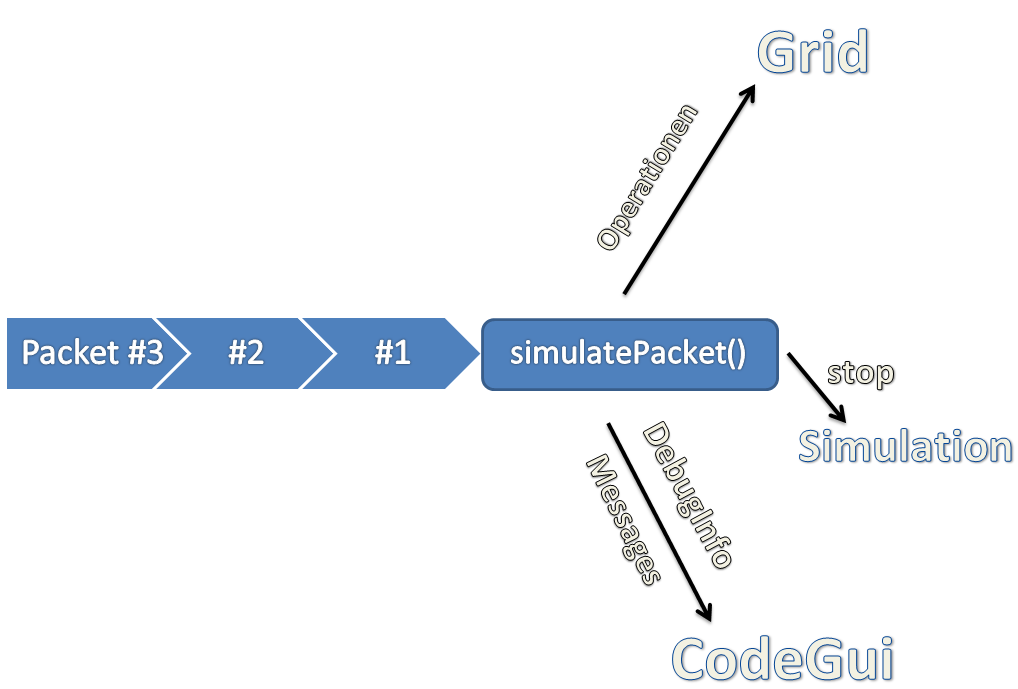
\includegraphics[scale=0.37]{client/socket-queue}
\end{frame}

\begin{frame}
\frametitle{CodeGUI}
\begin{center}
	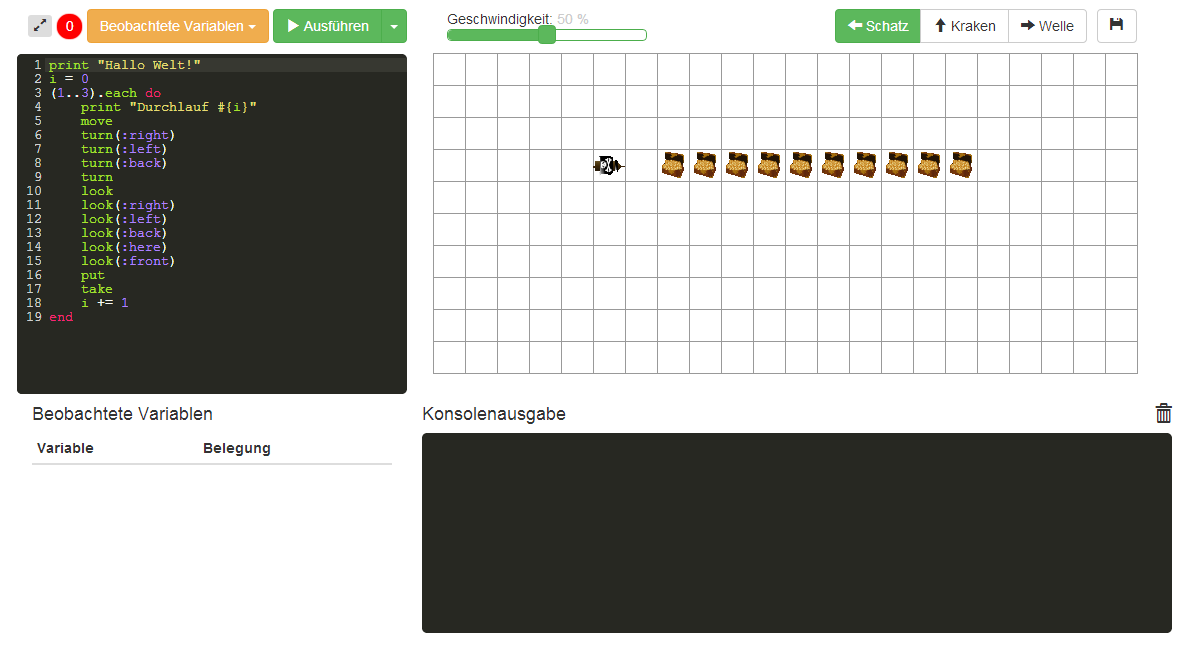
\includegraphics[scale=0.35]{client/client}
\end{center}
\end{frame}

\begin{frame}
\frametitle{Grid}
\begin{center}
	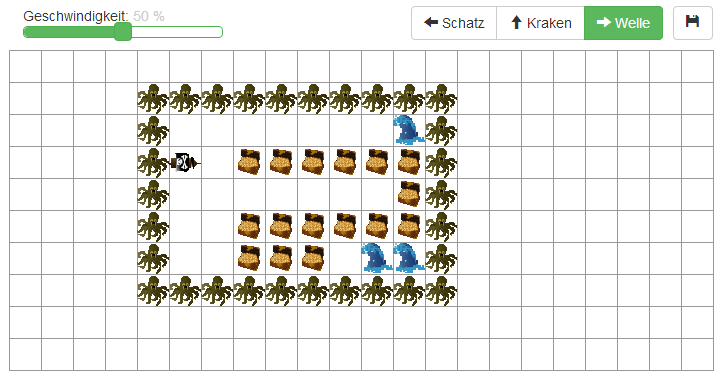
\includegraphics[scale=0.35]{client/grid} %TODO
\end{center}
\end{frame}

\begin{frame}
\frametitle{Modularität}
\begin{center}
	\inputminted[linenos, numbersep=2pt, tabsize=4]{javascript}{client/config.js}
\end{center}
\end{frame}
